% Options for packages loaded elsewhere
\PassOptionsToPackage{unicode}{hyperref}
\PassOptionsToPackage{hyphens}{url}
\PassOptionsToPackage{dvipsnames,svgnames,x11names}{xcolor}
%
\documentclass[
  letterpaper,
  DIV=11,
  numbers=noendperiod]{scrartcl}

\usepackage{amsmath,amssymb}
\usepackage{lmodern}
\usepackage{iftex}
\ifPDFTeX
  \usepackage[T1]{fontenc}
  \usepackage[utf8]{inputenc}
  \usepackage{textcomp} % provide euro and other symbols
\else % if luatex or xetex
  \usepackage{unicode-math}
  \defaultfontfeatures{Scale=MatchLowercase}
  \defaultfontfeatures[\rmfamily]{Ligatures=TeX,Scale=1}
\fi
% Use upquote if available, for straight quotes in verbatim environments
\IfFileExists{upquote.sty}{\usepackage{upquote}}{}
\IfFileExists{microtype.sty}{% use microtype if available
  \usepackage[]{microtype}
  \UseMicrotypeSet[protrusion]{basicmath} % disable protrusion for tt fonts
}{}
\makeatletter
\@ifundefined{KOMAClassName}{% if non-KOMA class
  \IfFileExists{parskip.sty}{%
    \usepackage{parskip}
  }{% else
    \setlength{\parindent}{0pt}
    \setlength{\parskip}{6pt plus 2pt minus 1pt}}
}{% if KOMA class
  \KOMAoptions{parskip=half}}
\makeatother
\usepackage{xcolor}
\setlength{\emergencystretch}{3em} % prevent overfull lines
\setcounter{secnumdepth}{-\maxdimen} % remove section numbering
% Make \paragraph and \subparagraph free-standing
\ifx\paragraph\undefined\else
  \let\oldparagraph\paragraph
  \renewcommand{\paragraph}[1]{\oldparagraph{#1}\mbox{}}
\fi
\ifx\subparagraph\undefined\else
  \let\oldsubparagraph\subparagraph
  \renewcommand{\subparagraph}[1]{\oldsubparagraph{#1}\mbox{}}
\fi


\providecommand{\tightlist}{%
  \setlength{\itemsep}{0pt}\setlength{\parskip}{0pt}}\usepackage{longtable,booktabs,array}
\usepackage{calc} % for calculating minipage widths
% Correct order of tables after \paragraph or \subparagraph
\usepackage{etoolbox}
\makeatletter
\patchcmd\longtable{\par}{\if@noskipsec\mbox{}\fi\par}{}{}
\makeatother
% Allow footnotes in longtable head/foot
\IfFileExists{footnotehyper.sty}{\usepackage{footnotehyper}}{\usepackage{footnote}}
\makesavenoteenv{longtable}
\usepackage{graphicx}
\makeatletter
\def\maxwidth{\ifdim\Gin@nat@width>\linewidth\linewidth\else\Gin@nat@width\fi}
\def\maxheight{\ifdim\Gin@nat@height>\textheight\textheight\else\Gin@nat@height\fi}
\makeatother
% Scale images if necessary, so that they will not overflow the page
% margins by default, and it is still possible to overwrite the defaults
% using explicit options in \includegraphics[width, height, ...]{}
\setkeys{Gin}{width=\maxwidth,height=\maxheight,keepaspectratio}
% Set default figure placement to htbp
\makeatletter
\def\fps@figure{htbp}
\makeatother
\newlength{\cslhangindent}
\setlength{\cslhangindent}{1.5em}
\newlength{\csllabelwidth}
\setlength{\csllabelwidth}{3em}
\newlength{\cslentryspacingunit} % times entry-spacing
\setlength{\cslentryspacingunit}{\parskip}
\newenvironment{CSLReferences}[2] % #1 hanging-ident, #2 entry spacing
 {% don't indent paragraphs
  \setlength{\parindent}{0pt}
  % turn on hanging indent if param 1 is 1
  \ifodd #1
  \let\oldpar\par
  \def\par{\hangindent=\cslhangindent\oldpar}
  \fi
  % set entry spacing
  \setlength{\parskip}{#2\cslentryspacingunit}
 }%
 {}
\usepackage{calc}
\newcommand{\CSLBlock}[1]{#1\hfill\break}
\newcommand{\CSLLeftMargin}[1]{\parbox[t]{\csllabelwidth}{#1}}
\newcommand{\CSLRightInline}[1]{\parbox[t]{\linewidth - \csllabelwidth}{#1}\break}
\newcommand{\CSLIndent}[1]{\hspace{\cslhangindent}#1}

\usepackage{booktabs}
\usepackage{longtable}
\usepackage{array}
\usepackage{multirow}
\usepackage{wrapfig}
\usepackage{float}
\usepackage{colortbl}
\usepackage{pdflscape}
\usepackage{tabu}
\usepackage{threeparttable}
\usepackage{threeparttablex}
\usepackage[normalem]{ulem}
\usepackage{makecell}
\usepackage{xcolor}
\KOMAoption{captions}{tableheading}
\makeatletter
\makeatother
\makeatletter
\makeatother
\makeatletter
\@ifpackageloaded{caption}{}{\usepackage{caption}}
\AtBeginDocument{%
\ifdefined\contentsname
  \renewcommand*\contentsname{Table of contents}
\else
  \newcommand\contentsname{Table of contents}
\fi
\ifdefined\listfigurename
  \renewcommand*\listfigurename{List of Figures}
\else
  \newcommand\listfigurename{List of Figures}
\fi
\ifdefined\listtablename
  \renewcommand*\listtablename{List of Tables}
\else
  \newcommand\listtablename{List of Tables}
\fi
\ifdefined\figurename
  \renewcommand*\figurename{Figure}
\else
  \newcommand\figurename{Figure}
\fi
\ifdefined\tablename
  \renewcommand*\tablename{Table}
\else
  \newcommand\tablename{Table}
\fi
}
\@ifpackageloaded{float}{}{\usepackage{float}}
\floatstyle{ruled}
\@ifundefined{c@chapter}{\newfloat{codelisting}{h}{lop}}{\newfloat{codelisting}{h}{lop}[chapter]}
\floatname{codelisting}{Listing}
\newcommand*\listoflistings{\listof{codelisting}{List of Listings}}
\makeatother
\makeatletter
\@ifpackageloaded{caption}{}{\usepackage{caption}}
\@ifpackageloaded{subcaption}{}{\usepackage{subcaption}}
\makeatother
\makeatletter
\@ifpackageloaded{tcolorbox}{}{\usepackage[many]{tcolorbox}}
\makeatother
\makeatletter
\@ifundefined{shadecolor}{\definecolor{shadecolor}{rgb}{.97, .97, .97}}
\makeatother
\makeatletter
\makeatother
\ifLuaTeX
  \usepackage{selnolig}  % disable illegal ligatures
\fi
\IfFileExists{bookmark.sty}{\usepackage{bookmark}}{\usepackage{hyperref}}
\IfFileExists{xurl.sty}{\usepackage{xurl}}{} % add URL line breaks if available
\urlstyle{same} % disable monospaced font for URLs
\hypersetup{
  pdftitle={Values from Lyrics: Pre-Registration},
  pdfauthor={Andrew M. Demetriou},
  colorlinks=true,
  linkcolor={blue},
  filecolor={Maroon},
  citecolor={Blue},
  urlcolor={Blue},
  pdfcreator={LaTeX via pandoc}}

\title{Values from Lyrics: Pre-Registration}
\author{Andrew M. Demetriou}
\date{}

\begin{document}
\maketitle
\ifdefined\Shaded\renewenvironment{Shaded}{\begin{tcolorbox}[frame hidden, enhanced, borderline west={3pt}{0pt}{shadecolor}, boxrule=0pt, interior hidden, breakable, sharp corners]}{\end{tcolorbox}}\fi

\hypertarget{study-information}{%
\subsection{Study Information}\label{study-information}}

\textbf{Contributors}: Andrew M. Demetriou, Jaehun Kim, Sandy Manolios,
Cynthia C.S. Liem

See Section~\ref{sec-contributions} for details of individual
contributions according to the
\href{https://www.kent.ac.uk/guides/credit-contributor-roles-taxonomy\#:~:text=CRediT\%20(Contributor\%20Roles\%20Taxonomy)\%20is,contribution\%20to\%20the\%20scholarly\%20output.}{Contributor
Roles Taxonomy}.\\

\hypertarget{overview}{%
\subsubsection{Overview}\label{overview}}

We aim to extend work that used natural language processing (NLP) to
estimate psychological values (e.g. (Schwartz et al. 2001)) in
social-media text (Ponizovskiy et al. 2020). Specifically we will
explore the potential to estimate the perceived psychological values in
song lyrics.

Our study primarily consists of comparisons between what people
indicate, and what NLP systems estimate, are the psychological values
expressed in song lyrics. We will gather responses from people using an
online survey. We will also use NLP systems to estimate the scores and
compare them to those from people.

As in Ponizovskiy et al. (2020) we estimate convergent validity of the
grouped NLP systems and our queztionnaire by estimating correlations
with related constructs measured using Linguistic Inquiry Word Count
(\href{https://liwc.app}{LIWC}; Boyd et al. (2022)). We will also
compare the performance of word counting methods used in Ponizovskiy et
al. (2020) with semantic distance methods similar to those used in e.g.
Beaty and Johnson (2021).

People who are exceptionally familiar or who have a strong preference
for song lyrics may give different ratings than others. To examine this
in the future, we also begin development of a psychometric questionnaire
aimed at measuring lyric preference intensity and expertise.

Lastly, we aim to make artifacts of this project reproducible. Thus,
reusable instances of the NLP systems will be available on
\href{https://replicate.com/eldrin/text-concept-similarity}{Replicate},
codebases and notebooks documenting our work will be available on
\href{https://https://github.com/andrew0302/values_from_lyrics}{Github},
as well as \href{https://osf.io/h87mz/}{Open Science Framework} which
will also include de-identified responses from participants. These
repositories will also contain the files we used to make our
\href{https://formR.org}{formR.org} survey, a test version of which can
be found \href{https://testmysurvey.formr.org/}{here}.

\hypertarget{sec-hypotheses}{%
\subsubsection{Hypotheses}\label{sec-hypotheses}}

As this is an initial study, our hypotheses are not severe:

\textbf{Primary Hypothesis}: Grouped NLP systems show a statistically
significant correlation with grouped \textbf{a)} participant ratings
across all 10 personal values, and \textbf{b)} with related LIWC
constructs - in the same or greater magnitude as shown in Ponizovskiy et
al. (2020).

\textbf{Primary Null Hypothesis}: Grouped NLP systems show no evidence
of a correlation with participant ratings across all 10 personal values,
or LIWC constructs.

\textbf{Secondary Hypothesis}: Magnitude of these correlations will be
lower with word-counting methods than with semantic distance methods.

\textbf{Secondary Null Hypothesis}: Magnitude of these correlations show
no difference.

\hypertarget{study-type}{%
\subsubsection{Study Type}\label{study-type}}

Observational study - Data is collected from study participants that are
not randomly assigned to a treatment.

\hypertarget{blinding}{%
\subsubsection{Blinding}\label{blinding}}

No blinding is involved in this study

\hypertarget{design-plan}{%
\subsection{Design Plan}\label{design-plan}}

\hypertarget{participant-recruitment-platform}{%
\subsubsection{Participant Recruitment
Platform}\label{participant-recruitment-platform}}

We will recruit a U.S. representative sample of participants from
\href{https://prolific.co}{Prolific.co}.

\hypertarget{survey-platform}{%
\subsubsection{Survey Platform}\label{survey-platform}}

Our primary measure is the perceived presence of personal values in song
lyrics. Song lyrics may be written from the perspective of the author,
but also from the perspective of someone or something else - sometimes
referred to as the `speaker'. As we are measuring the presence of values
as suggested in the lyrics themselves, we explicitly ask participants to
respond with the perspective of the \emph{speaker} in mind, and not the
author.

The survey will be implemented on an instance of
\href{https://formR.org}{formR.org} hosted on the servers of
\href{https://www.tudelft.nl/}{Delft University of Technology} to ensure
GDPR compliance. A test version of the survey can be found
\href{https://testmysurvey.formr.org/}{here}. The \texttt{.csv} survey
files used as input to formR were constructed in R\footnote{see
  \texttt{survey\_builder\_*.Rmd} notebook in the
  \texttt{IV\_survey\_builder} folder of this repository.}. The main
component of the survey involves showing participants the lyrics to a
number of songs, one at a time. For each song they are asked to respond
to set of questions designed to assess the presence of values in the
lyrics.

The majority of items require a Likert-type response. In order to gather
a more continuous measure, we used a slider with no starting point: the
\texttt{rating\ button} option in formR shows a horizontal gray bar with
two labeled poles (e.g.~agree - disagree). For each value there is a
brief description, followed by the slider labelled (``opposed to their
values'' - ``of supreme importance'').

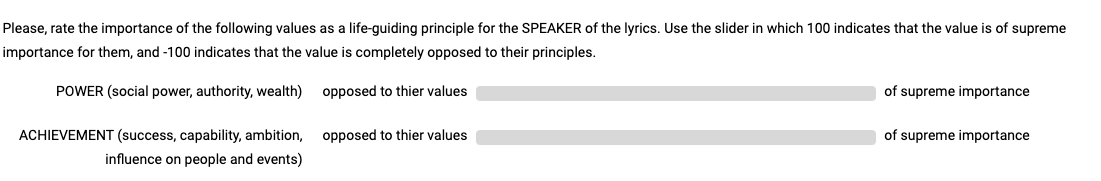
\includegraphics{screenshots/formR.png}

Participants are instructed to indicate on the bar the degree to which
they e.g.~agree or disagree, as they might with a slider. However, the
gray bar has no visible slider, thus no starting value. Although it
shows no divisions it contains 20 subdivisions. To ensure that
participants understand the use of this method, we include a `training
and explanation' page at the beginning of our
\href{https://testmysurvey.formr.org/}{survey}.

\hypertarget{randomization}{%
\paragraph{Randomization}\label{randomization}}

Participants are randomly assigned 18 lyric stimuli to rate. We
experienced issues with the formR platform when the number of lyric
stimuli in the survey was greater than 60. Thus, our stimulus set will
be separated into otherwise identical survey files on the formR server,
with no more than 60 lyrics in each survey file. Participants will be
randomly assigned to one of the surveys, which will in turn randomly
select a subset of stimuli to be rated.

\hypertarget{survey-measures}{%
\subsubsection{Survey Measures}\label{survey-measures}}

\hypertarget{personal-values}{%
\paragraph{Personal Values}\label{personal-values}}

Prior research (e.g. Schwartz et al. (2001)) has shown evidence for the
presence of personal values as guiding principles in the lives of
people. Participants will indicate the degree to which they think 10
values are present for each set of lyrics that they are shown. We chose
to use the Short Schwarz's Value Survey Lindeman and Verkasalo (2005) as
it is the briefest instrument whose reliability and validity has been
shown to be adequate, to our knowledge. The original instrument displays
a brief definition of each of the ten values in the Schwartz inventory,
(e.g.~``POWER (social power, authority, wealth)'') and asks participants
to indicate on a Likert scale (0= Opposed to my principles, 8 = Of
supreme importance) the degree of importance of the value to them. In
our version, participants will indicate on a solid gray bar as described
above. As our participants will be rating a stimulus that is not
themselves, we adjusted the wording slightly: e.g.~``Please, rate the
importance of the following values as a life-guiding principle for the
SPEAKER of the lyrics.''

\hypertarget{lyric-preferences}{%
\paragraph{Lyric Preferences}\label{lyric-preferences}}

To assess whether expertise in lyrics or a preference for lyrical
content has an effect on the ratings given, we have begun developing a
scale, partially inspired by the Preference Intensity scale in Schäfer
and Sedlmeier (2009). Our original ad-hoc scale consisted of 10
Likert-type items. Participants in our second pilot (see
Section~\ref{sec-pilot2}) were asked to respond to the 10 items, and to
an additional `open response' format item that asked: ``Can you think of
any other activities or indications that someone has an affinity for
song lyrics? If so, please enter them here:''. We removed poorly
performing items, and added 5 items based on participant responses to
the open format question. As this instrument has yet to show
satisfactory reliability or validity, we will continue adding and
removing items using factor analysis and item response theory techniques
as we progress.

\hypertarget{additional-measures}{%
\paragraph{Additional Measures}\label{additional-measures}}

\hypertarget{familiarity}{%
\subparagraph{Familiarity}\label{familiarity}}

To control for familiarity of the lyrics, we will ask participants to
indicate (yes/no) if they recognize the song that the lyrics came from.
In addition, we will ask the participants whether or not they think the
speaker and writer are the same person as an exploratory measure.

\hypertarget{rating-confidence}{%
\subparagraph{Rating Confidence}\label{rating-confidence}}

It has been suggested that a rater's confidence in their annotation is a
relevant indicator of reliability (although possibly orthogonal to
accuracy; see Cabitza, Campagner, and Sconfienza (2020)). For each set
of lyrics, we will ask participants to indicate the degree to which they
are confident in their ratings on a solid bar ranging from `Extremely
unconfident' to `Extremely confident').

Our pilot study (Section~\ref{sec-pilot2}) of 20 lyric stimuli suggests
participants are overall `Somewhat confident' in their responses, which
provides some initial evidence of self-perceived intra-rater reliability
of our procedure.

\begin{figure}

{\centering 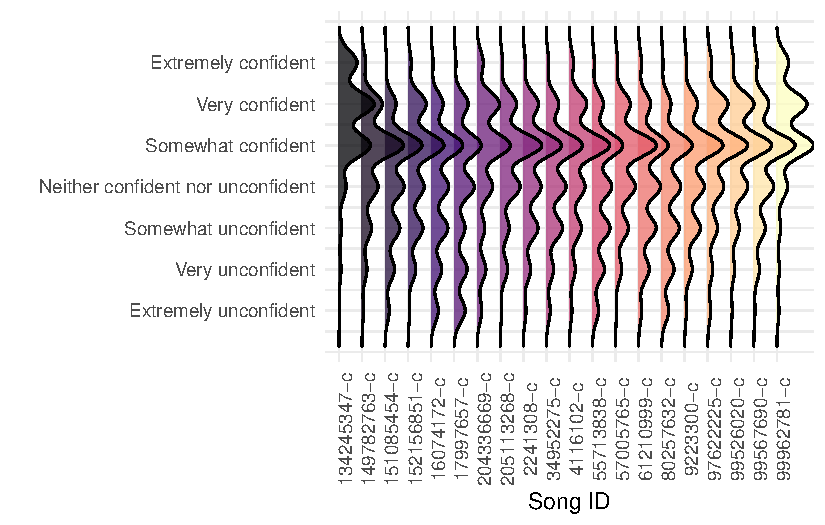
\includegraphics{pre-registration_pdf_files/figure-pdf/fig-1-1.pdf}

}

\caption{\label{fig-1}Participant self-ratings of Confidence in own
responses for 20 lyric stimuli}

\end{figure}

\hypertarget{sec-sampling}{%
\subsubsection{Sampling Procedures}\label{sec-sampling}}

\hypertarget{lyric-stimulus-set}{%
\paragraph{Lyric Stimulus Set}\label{lyric-stimulus-set}}

We aim to annotate a total of 360 lyric stimuli drawn from a pool of
2200, with approximately 25 ratings for each. This is not intended to be
a fully representative sample, but rather a sufficiently large sample
with which to examine the potential of our procedure. Size limits were
determined by estimating the smallest sample size to demonstrate the
viability of our procedure, taking into account time and budgetary
constraints of the research team.

Our 360 stimulus set was derived using stratified random sampling (see
Section~\ref{sec-stratifiedsampling} for details), and then a final
manual screening by the research team (see
Section~\ref{sec-manualscreening}).

The overall population of song lyrics was derived from the Spotify
Million Playlist Dataset
\href{https://aicrowd.com/challenges/spotify-million-playlist-dataset-challenge}{MPD}
which contains 1 million Spotify user-generated playlists, chosen
because of its size and its recency vs.~other similar datasets.

The lyric stimuli were drawn from the database of
\href{https://musixmatch.com}{musiXmatch} using their API, which
provides approximately 30\% of the lyrics of each song.

\hypertarget{number-of-ratings}{%
\paragraph{Number of ratings}\label{number-of-ratings}}

\hypertarget{task-subjectivity}{%
\subparagraph{Task Subjectivity}\label{task-subjectivity}}

It may be the case that the number of raters required to reach a
satisfactory inter-rater reliability increases with the degree to which
the task is subjective. Thus, at the very end of the survey we will ask
participants to indicate the degree to which they found the task to be
subjective on a solid bar ranging from `Completely subjective' to
`Completely objective'). The mode of responses in our pilot study (see
Section~\ref{sec-pilot2}) suggests participants find the task to be
`Very Subjective'. Thus we expect we will need a relatively large number
of ratings per lyric stimulus for our study.

\begin{figure}

{\centering 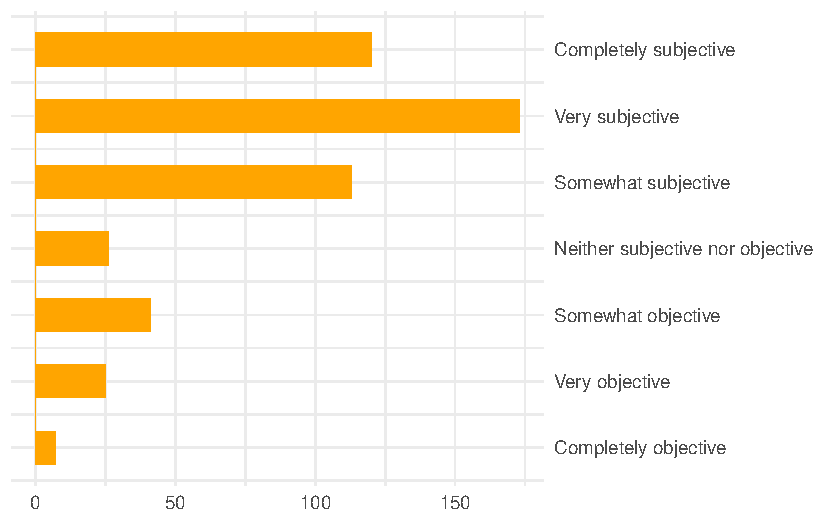
\includegraphics{pre-registration_pdf_files/figure-pdf/fig-2-1.pdf}

}

\caption{\label{fig-2}Participant ratings of subjectivity of the lyric
rating task.}

\end{figure}

We followed a procedure inspired by DeBruine and Jones (2018) to
determine the number of ratings per lyric stimulus. Specifically, we
chose a small subset of 20 lyric samples, and had approximately 500
participants rate them all. We then randomly sub-sampled from the pool
of 500 raters in increments ranging from 5 to 50 raters, and estimated
Cronbach's alpha for each subsample. Our conclusions suggested
conservative estimates of 25 raters per lyric stimulus. See
Section~\ref{sec-pilot2} for details.

\hypertarget{number-of-participants}{%
\paragraph{Number of Participants}\label{number-of-participants}}

We estimated how long it would take a participant to complete our lyrics
questionnaire, and the time it would take to complete all questions for
a single lyric stimulus on average. Data were collected during our
second pilot (see Section~\ref{sec-pilot2}).

\hypertarget{tbl-2}{}
\begin{table}
\caption{\label{tbl-2}Time in seconds per lyric stimulus }\tabularnewline

\centering
\begin{threeparttable}
\begin{tabular}{l|r|r|r}
\hline
outliers & mean & median & sd\\
\hline
no outliers removed & 40.34782 & 30.4965 & 43.49806\\
\hline
outliers set at < 900 & 39.94714 & 30.4850 & 35.46503\\
\hline
\end{tabular}
\begin{tablenotes}[para]
\item \textit{Note: } 
\item Mean, median and standard deviation time in *seconds* per lyric stimulus determined by subtracting time at the first click in a block of questions from the last click for each song.
\end{tablenotes}
\end{threeparttable}
\end{table}

We aimed for a 30-minute survey. We estimated conservatively that it
would take approximately 85 seconds to complete each lyric stimulus
item, and approximately 3 minutes (240 seconds) to complete the other
items in the survey. Thus we had room for 18 lyric stimulus items.

Given the total of 360 lyric stimuli and the time taken per stimulus, we
estimated the number of participants necessary to receive approximately
25 ratings per stimuli using simulation \footnote{see
  \texttt{IX\_participation\_estimation.ipynb} notebook in
  \texttt{II\_rater\_pilot} folder}. We thus expect to collect data for
530 participants. See Section~\ref{sec-participantsimulation} for
further details.

\hypertarget{natural-language-processing}{%
\subsubsection{Natural Language
Processing}\label{natural-language-processing}}

\hypertarget{lexicon}{%
\paragraph{Lexicon}\label{lexicon}}

We will use the \texttt{Refined\_dictionary.txt} file, included in the
supplementary materials of Ponizovskiy et al. (2020) stored on the
\href{https://osf.io/vy475/}{Open Science Framework}.

\hypertarget{pre-trained-models}{%
\paragraph{Pre-trained models}\label{pre-trained-models}}

We consider two commonly used pre-trained word-embedding models:
\texttt{word2vec-google-news} is trained on a corpus of online news
articles, including about 100 billion words. It is based on the work of
Mikolov et al. (2013). \texttt{GloVe-common-crawl-840B} is trained with
the model suggested by Pennington, Socher, and Manning (2014) using
crawled large-scale web pages, including about 840 billion words.

\hypertarget{models-we-trained}{%
\paragraph{Models we trained}\label{models-we-trained}}

We will also consider word embedding models directly trained from the
lyrics corpus, based on Pennington, Socher, and Manning (2014). We
select models on two sets of off-line criteria:

\begin{enumerate}
\def\labelenumi{\arabic{enumi}.}
\tightlist
\item
  loss function on the hold-out data set and
\item
  English word similarity judgment data employed from Faruqui and Dyer
  (2014).
\end{enumerate}

\hypertarget{word-vector-aggregation}{%
\paragraph{Word-vector aggregation}\label{word-vector-aggregation}}

It is necessary to aggregate word vectors from each lyric into a single
lyric vector, which is then compared to sets of words belonging to each
value. We consider two methods: 1) uniform average and 2) weighted sum.
In particular, weighted sum employs the inverse-document-frequency for
weighting each word vector within the lyrics De Boom et al. (2016).

\hypertarget{analytic-approach}{%
\subsubsection{Analytic approach}\label{analytic-approach}}

Our primary hypothesis is that we will observe a correlation in ratings
between participants and output from NLP systems (see
Section~\ref{sec-hypotheses} and Section~\ref{sec-magnitudes}).

Estimating a `ground truth' for each lyric stimulus from participant
ratings is non-trivial. Specifically, participants will use our survey
instrument differently (e.g.~some will give overall more extreme scores,
whereas some will more consistently give scores close to the middle of
the slider bar). We therefore aim to estimate scores for stimuli while
statistically controlling for the effect of participant's tendency to
use the survey.

\begin{figure}

{\centering 

\begin{figure}[H]

{\centering 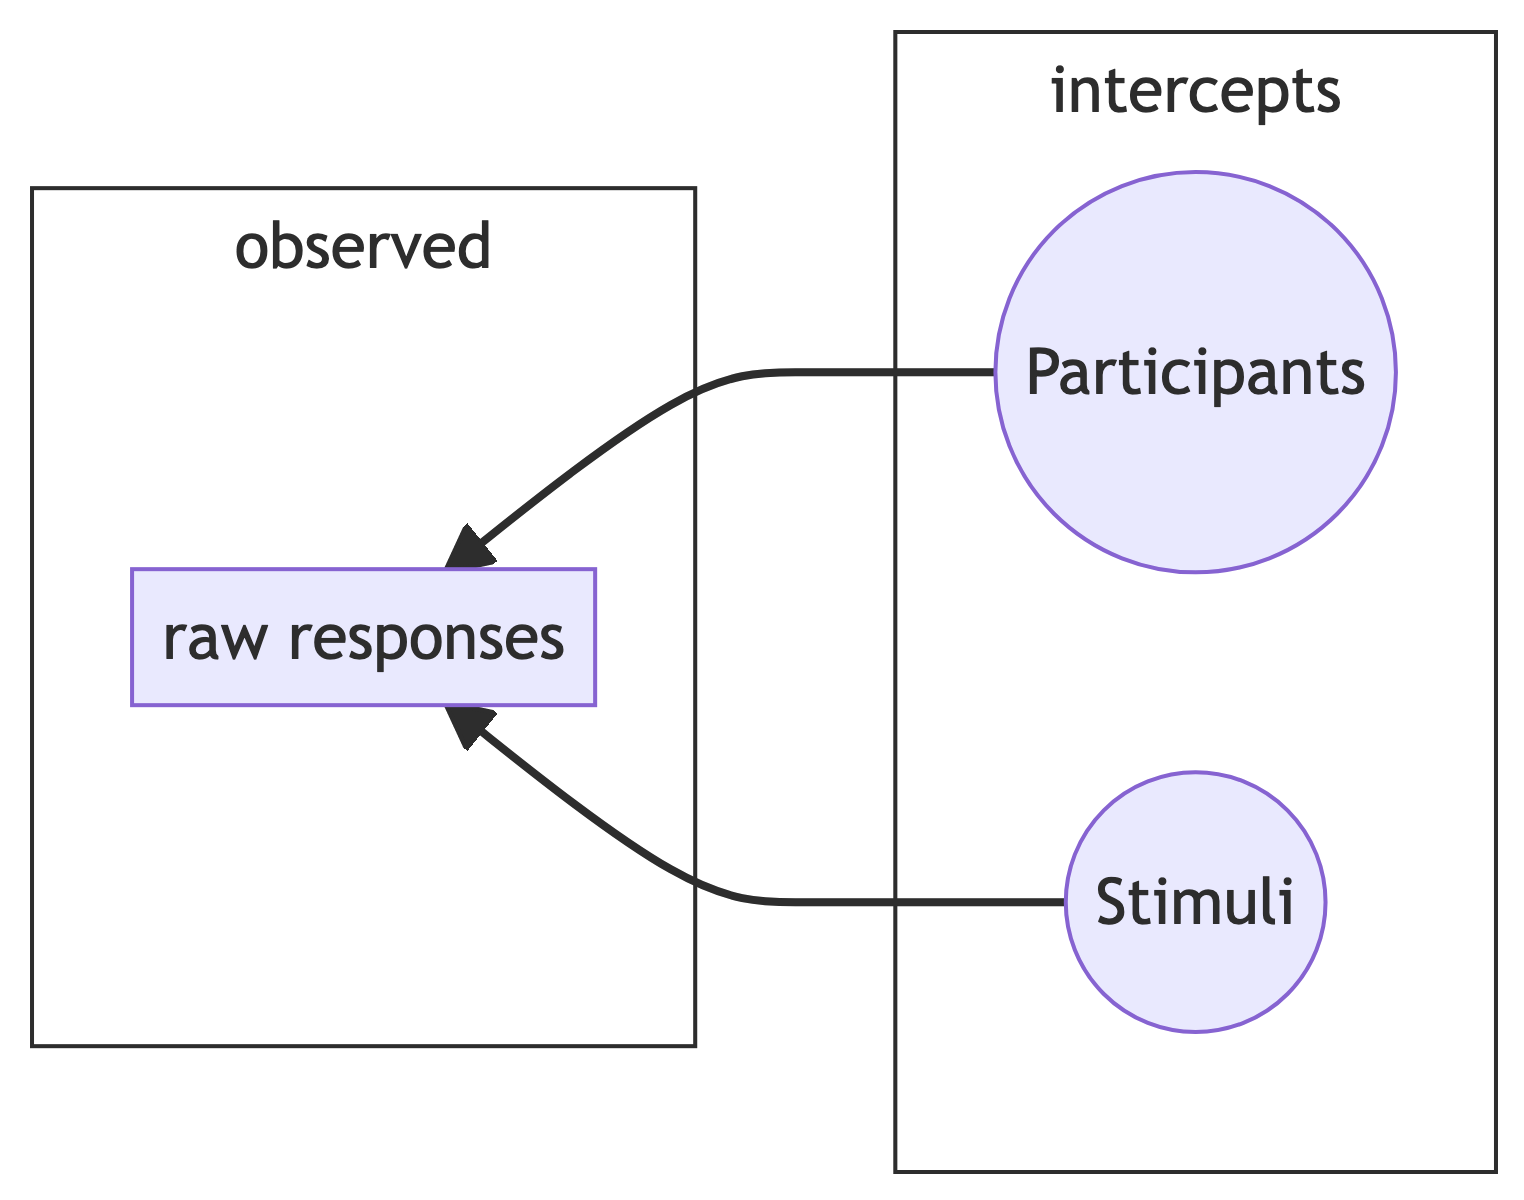
\includegraphics[width=3.98in,height=3.14in]{pre-registration_pdf_files/figure-latex/mermaid-figure-1.png}

}

\end{figure}

}

\caption{\label{fig-4}Cross-classified model, with intercepts estimated
for individual participants and individual lyric stimuli}

\end{figure}

We take a cross-classified approach, whereby we attempt to explicitly
model the tendency of participant use of the survey by estimating a
\texttt{participant\ intercept} for each one. Our primary analysis
involves correlating the \texttt{stimuli\ intercept}\footnote{We refer
  to this as the ``item intercept'' in our notebooks. See folder
  \texttt{III\_simulation\_study} for further details.} with output for
automated systems.

Similar to Beaty and Johnson (2021), the ratings from different NLP
systems will be linearly combined into a latent variable for each value.
These are then correlated to the \texttt{stimuli\ intercepts}.

\begin{figure}

{\centering 

\begin{figure}[H]

{\centering 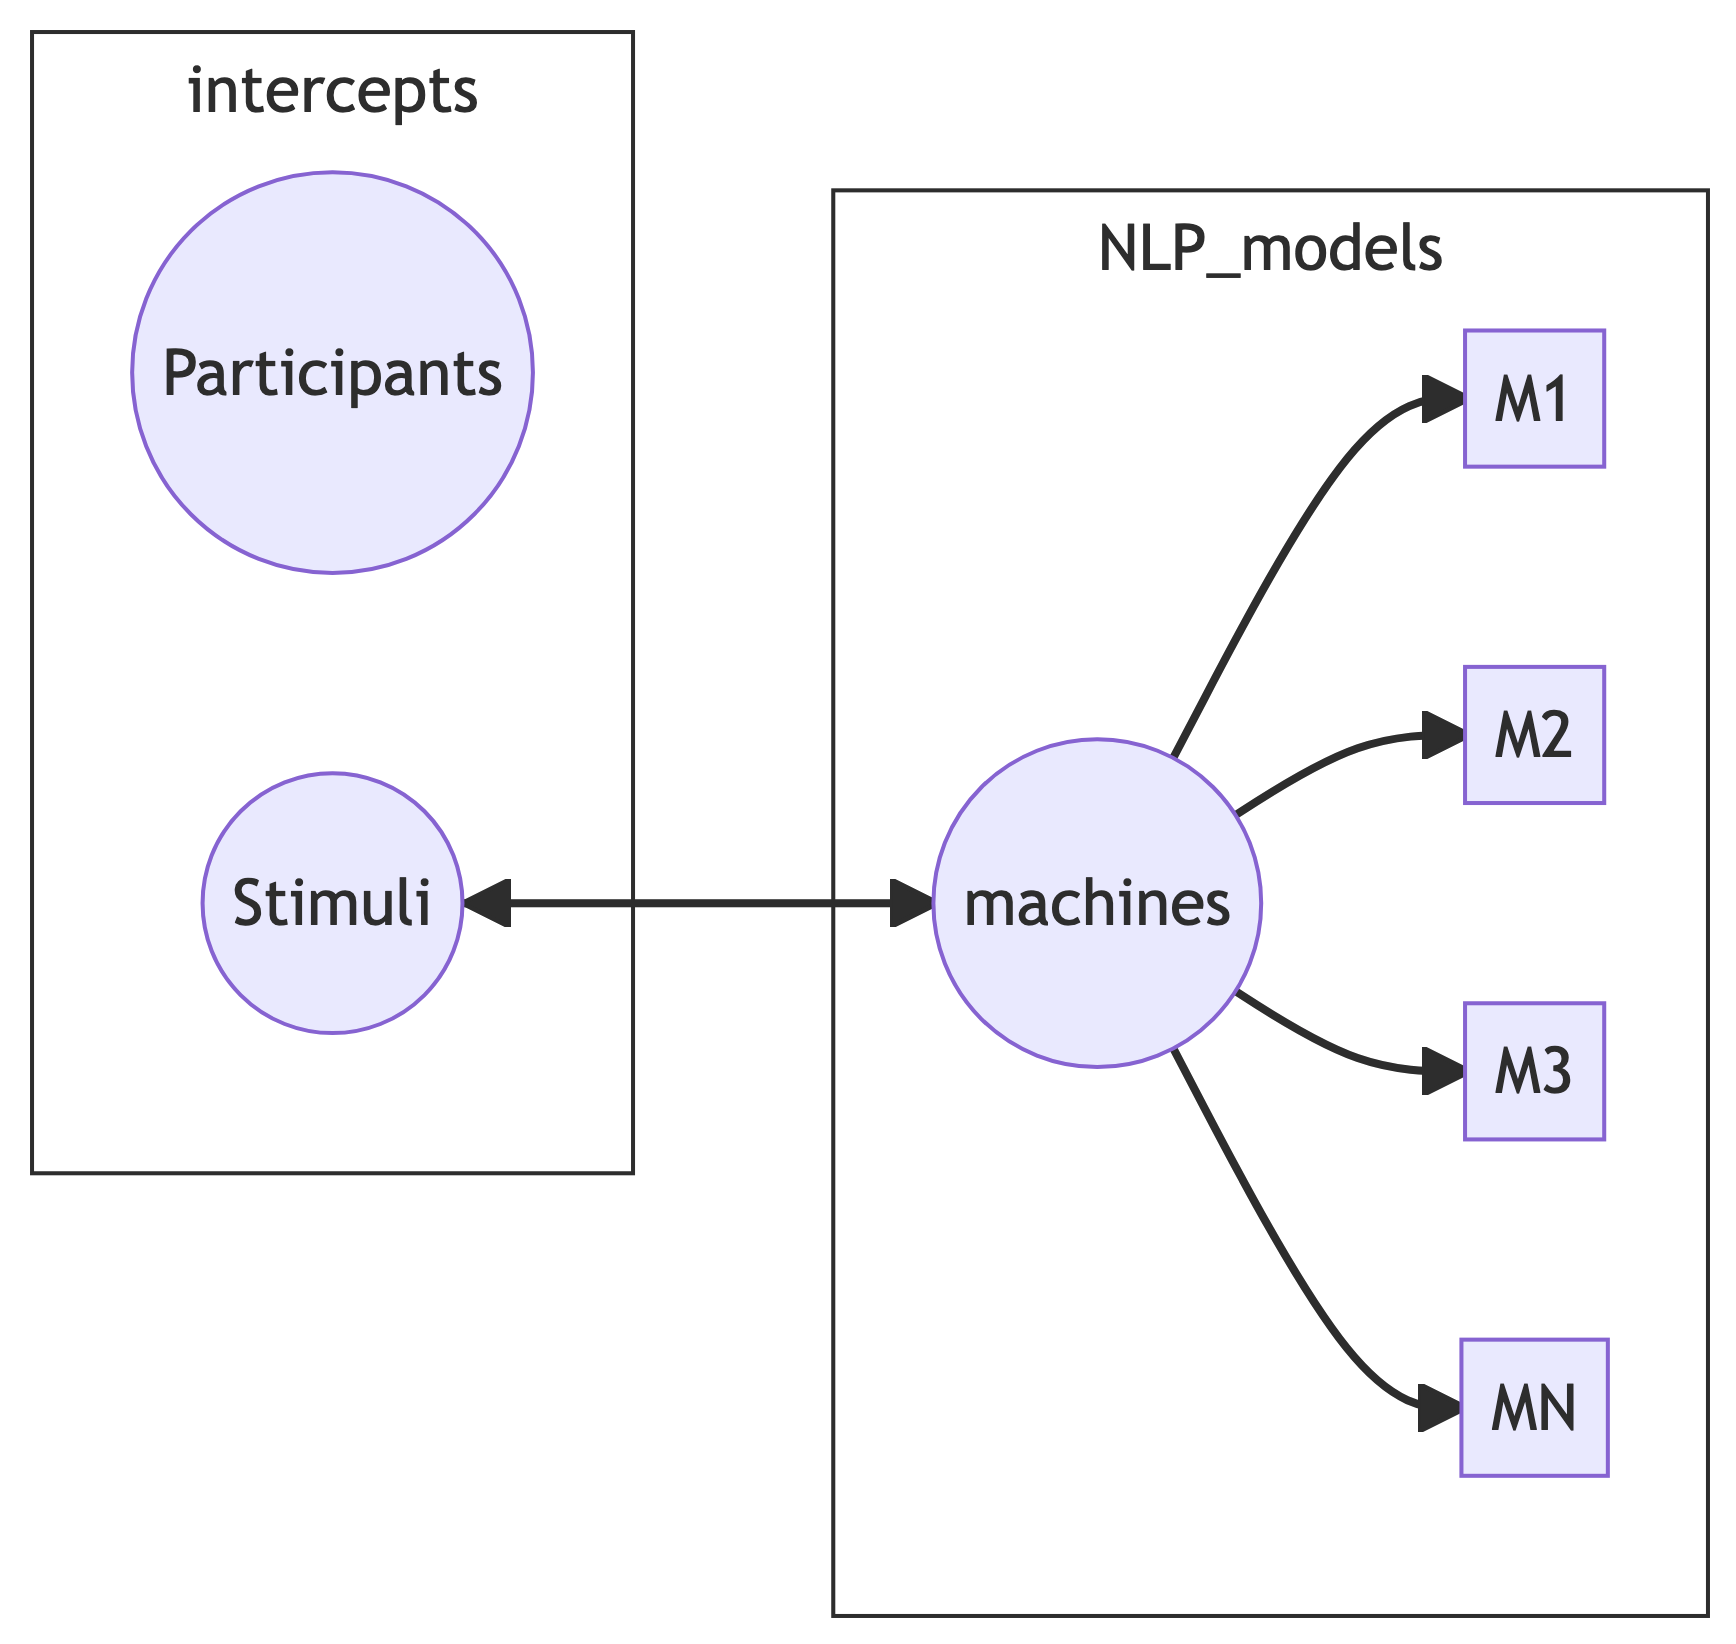
\includegraphics[width=4.53in,height=4.29in]{pre-registration_pdf_files/figure-latex/mermaid-figure-2.png}

}

\end{figure}

}

\caption{\label{fig-5}Latent variable representing ratings from multiple
NLP Systems}

\end{figure}

We will use the proprietary software,
\href{https://www.statmodel.com}{Mplus} to estimate the
models\footnote{We built our analysis models using simulated data. We
  explain the models we will use in the \texttt{III\_simulation\_study}
  folder}.

\hypertarget{contributions}{%
\subsubsection{Contributions}\label{contributions}}

We extend existing work primarily in three ways: Firstly, we examine
whether the work in Ponizovskiy et al. (2020) can be extended to song
lyrics: Ponizovskiy et al. (2020) showed evidence of validity for a
lexicon of words for measuring a set of 10 personal values in
social-media text.

Secondly, we compare semantic distance (the degree to which words are
related) estimated using NLP systems to the results of word counting.
Prior studies have counted the number of times specific words from a
fixed lexicon were used in a given body of text as a means of measuring
psychological constructs Ponizovskiy et al. (2020). However, song lyrics
may not contain those exact words, and may instead use synonymous or
otherwise meaningfully similar words, or even slang and metaphors. Our
method allows for more word coverage: rather than count words from a
fixed lexicon, we will estimate the semantic distance between the words
in the lexicon that represent each personal value, and the song lyrics
in order to derive a score for each value.

Thirdly, we linearly combine the output of multiple NLP systems into a
single latent variable, to represent the shared variance of the machine
ratings: as each NLP system is developed using 1) an algorithm trained
on 2) a corpus, each algorithm/corpus combination will estimate the
semantic distance between two words differently. This loosely parallels
how human participants may rate each set of lyrics differently. Beaty
and Johnson (2021) showed that this latent variable of semantic distance
estimations resulted in overlap with a latent variable of human ratings
as high as r = .9, albeit in a different domain. This approach further
allows us to estimate the contribution of each algorithm / corpus setup
to the shared variance.

We further contribute three assets: firstly, we provide containerized,
API-reachable interface to the models that we used to estimate semantic
similarity, housed on
\href{https://replicate.com/eldrin/text-concept-similarity}{Replicate}.
Secondly, we share code notebooks written with the intention of allowing
for reproducibility, replication, and extension of our work. Thirdly, we
share the beginnings of a psychometric scale for assessing lyric
preference intensity and expertise (Section~\ref{sec-lyricquestions}).

\hypertarget{appendix}{%
\section{Appendix}\label{appendix}}

\hypertarget{sec-magnitudes}{%
\subsection{a) hypothesized magnitudes}\label{sec-magnitudes}}

\begin{itemize}
\item
  LIWC correlations with participant ratings of Personal Values
  \footnote{see table 2 in Ponizovskiy et al. (2020)}:

  \begin{itemize}
  \tightlist
  \item
    liwc insight with self-direction, .43
  \item
    liwc sexuality with hedonism, .13
  \item
    liwc achievement with achievement .47
  \item
    liwc power with power, .19
  \item
    liwc power with conformity, .16
  \item
    liwc risk with security, .32
  \item
    liwc religion with traditionalism, .79
  \item
    liwc family with benevolence, .57
  \end{itemize}
\end{itemize}

\begin{itemize}
\item
  Correlations of self ratings of Personal Values with automated
  estimates from essays \footnote{see table 4 in Ponizovskiy et al.
    (2020)}:

  \begin{itemize}
  \tightlist
  \item
    self-direction: .23
  \item
    stimulation: .12
  \item
    hedonism: .22
  \item
    achievement: .17
  \item
    power: -.02
  \item
    security: .00
  \item
    conformity: .07
  \item
    tradition: .31
  \item
    benevolence: .18
  \item
    universalism: .29
  \end{itemize}
\end{itemize}

\hypertarget{b-number-of-ratings-per-stimulus}{%
\subsection{b) number of ratings per
stimulus}\label{b-number-of-ratings-per-stimulus}}

We conducted two pilot studies to estimate the number of ratings needed
for each song lyric.

\hypertarget{sec-pilot1}{%
\subsubsection{Pilot 1}\label{sec-pilot1}}

Our first pilot study aimed to gather an tentative estimate of the time
it would take participants to complete components of the survey using a
small convenience sample. We recruited participants first on
\href{https://www.reddit.com/r/SampleSize}{reddit.com} and then from
within the lab of the research team. Participants were shown four lyric
stimuli and asked to complete our adapted personal values questionnaire
for each song lyric. we used the Qualtrics platform to create and host
the survey (\href{https://www.qualtrics.com}{qualtrics.com}).

\hypertarget{tbl-1}{}
\begin{table}
\caption{\label{tbl-1}Time in minutes to complete task. }\tabularnewline

\centering
\begin{threeparttable}
\begin{tabular}{l|r|r|r|r|r}
\hline
statistic & lyric preferences & song 1 & song 2 & song 3 & song 4\\
\hline
mean & 1.4460848 & 2.019053 & 1.626731 & 1.374369 & 1.072906\\
\hline
sd & 0.7674326 & 1.572428 & 1.742973 & 1.480763 & 1.053221\\
\hline
\end{tabular}
\begin{tablenotes}[para]
\item \textit{Note: } 
\item Time in minutes determined by subtracting time at the first click in a block of questions from the last click, and dividing by 60.
\end{tablenotes}
\end{threeparttable}
\end{table}

On average participants took 1.52 minutes per song. However,
Table~\ref{tbl-1} shows that the time to complete the items per song
decreased as participants progressed through the questionnaires. Thus we
estimated that questions for 20 stimuli could be completed in
approximately 30 minutes.

\hypertarget{sec-pilot2}{%
\subsubsection{Pilot 2}\label{sec-pilot2}}

Following our first pilot (Section~\ref{sec-pilot1}), we aimed to
estimate the smallest number of ratings necessary to achieve a
satisfactory inter-rater reliability. We recruited in proportions for a
representative sample of the United States on the
\href{https://www.prolific.co}{Prolific.co} participant recruitment
platform.We gathered responses from 500 participants on 20 lyric
stimuli, and the followed a similar procedure as described in DeBruine
and Jones (2018). For each of the 10 values, we estimated Cronbach's
alpha for a range of subsample sizes, ranging from 5 to 50 participants
in increments of 5. This procedure was repeated 10 times per increment,
separately for each of the 10 values. We then examined the distribution
of Cronbach's Alpha for each of the 10 personal values to determine the
frequency with which it exceeded a threshold of .7, commonly considered
to be an acceptable level of reliability.

The distributions of Cronbach's Alpha estimates for the value of
Stimulation are shown in Figure~\ref{fig-3}, and suggested the need for
more than 25 raters to consistently achieve a Cronbach's Alpha greater
than .7. We thus conclude that a conservative estimate for the number of
ratings is 25.

\begin{figure}

{\centering 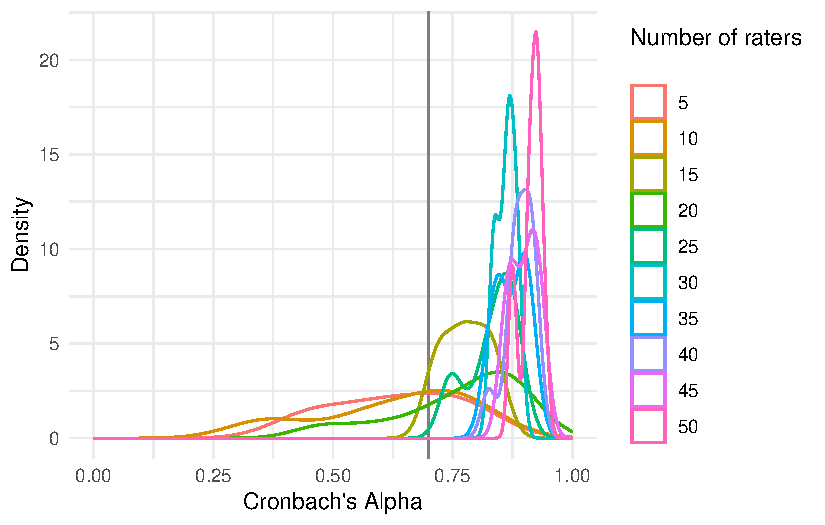
\includegraphics{pre-registration_pdf_files/figure-pdf/fig-3-1.pdf}

}

\caption{\label{fig-3}Distribution of Cronbach's Alpha estimates for the
value of Stimulation, by sub-sample size}

\end{figure}

\hypertarget{sec-lyricquestions}{%
\subsection{c) lyric preference and expertise
questionnaire}\label{sec-lyricquestions}}

This questionnaire remains a work in progress; we include the current
version as of this pre-registration.

\begin{enumerate}
\def\labelenumi{\arabic{enumi}.}
\tightlist
\item
  I prefer music that contains lyrics, as opposed to music that does not
\item
  I only pay attention to the lyrics of songs or artists that I like
\item
  I always pay attention to the lyrics of a song, if the song has them
\item
  I enjoy learning about song lyrics and their meaning, for example by
  reading blogs and forums or listening to artist interviews
\item
  If a song has lyrics that I don't like for any reason, I don't listen
  to it
\item
  If I am not sure about the lyrics of a song, I look them up
\item
  I contribute to online resources on lyrics (e.g.~on forums, or on
  platforms where I can contribute lyric transcriptions)
\item
  I memorize the lyrics to the songs I listen to
\item
  I write my own song lyrics
\item
  I post excerpts of song lyrics online, e.g.~on social media
\item
  I discuss song lyrics with my friends
\item
  I come up with alternate versions of song lyrics that I find
  entertaining, i.e.~song parodies
\item
  I ponder the meaning of lyrics
\item
  I quote lyrics in conversation
\item
  I read and/or write poetry
\item
  What percentage of your music library do you think contains songs with
  lyrics?
\end{enumerate}

\hypertarget{sec-stratifiedsampling}{%
\subsection{d) stratified sampling for stimulus
set}\label{sec-stratifiedsampling}}

Our sampling process was as follows:

\begin{enumerate}
\def\labelenumi{\arabic{enumi}.}
\tightlist
\item
  uniformly sub-sample 60k artists out of 300k artists in the MPD
\item
  determine song availability on musiXmatch using their API
\item
  create a large pool of available songs for the 60k artists
\end{enumerate}

We then consider four aspects of lyric data as strata for random
sampling:

\begin{enumerate}
\def\labelenumi{\arabic{enumi}.}
\tightlist
\item
  Genre, estimated using topic modeling on artist-tags (Schindler et
  al., 2012)
\item
  Popularity, estimated via artist playlist frequency
\item
  Lyric Topic, estimating using topic modeling
\item
  Release date
\end{enumerate}

Estimated genre and lyric topic resulted in categorical groupings.
Popularity and Release date were divided into equally spaced sub-ranges;
e.g.~we divided release year into decades (60s, 70s, 80s, and so on).

\hypertarget{bias-correction}{%
\subsubsection{bias correction}\label{bias-correction}}

We expect our dataset will lean towards songs that are a) recent, and b)
popular. Specifically, our continuous strata variables are separated
into bins, and we expect that some bins in the defined strata will
result in very few songs. Thus, we compensate by oversampling the less
populated bins. To do so, we employ the maximum-a-posteriori (MAP)
estimate of the parameter of the categorical distribution for each
stratum: this inflates the probability that songs from the less
populated bins will be selected. The procedure is controlled by a free
parameter ``alpha,'' which determines the degree to which we inflate the
bins. However, we do not know any prior study that suggests an
appropriate alpha that suits our study context. Thus, we heuristically
set the parameter to 40,000, which implies that songs in the lesser bins
will comprise 5 - 10\% of the resulting pool.

The total number of samples was set at 2,200 based on estimations of the
research team as to the maximum possible number of songs that could be
rated in this study given time and budget constraints.

Further, we select the samples as a dynamic search process rather than a
typical sampling procedure:

\begin{enumerate}
\def\labelenumi{\arabic{enumi}.}
\tightlist
\item
  Set ``reference distribution'' for each stratum, and an empty dataset
  to populate:

  \begin{enumerate}
  \def\labelenumii{\alph{enumii})}
  \tightlist
  \item
    each reference distribution is the original distribution compensated
    by MAP with alpha = 40,000
  \item
    set the total number of samples (\emph{N}=2200) to be found
  \item
    define \emph{B} as a currently empty set of lyrics which we will
    populate
  \end{enumerate}
\item
  Repeat the following until the number of samples in B reaches N:

  \begin{enumerate}
  \def\labelenumii{\alph{enumii})}
  \tightlist
  \item
    select a stratum uniformly randomly
  \item
    select a song such that the distribution of samples in \emph{B} most
    closely resembles reference distribution
  \item
    add song to \emph{B}
  \end{enumerate}
\end{enumerate}

From the very first lyric stimulus selected, this procedure will allow
for any length of slice of \emph{B} to approximately follow the
reference distribution for each stratum. We expect that this procedure
can be useful 1) when the first few items must follow the reference
distribution and 2) when there is the possibility of continuing the
annotation project at a later time, and thus the sampling procedure must
be continued rather than starting anew.

\hypertarget{sec-manualscreening}{%
\subsection{e) manual screening procedure}\label{sec-manualscreening}}

Lyrics of the stimulus set were then manually screened to see if they
were a match to the actual song \footnote{see
  \texttt{I\_lyric\_checker*.Rmd} in the \texttt{IV\_survey\_builder}
  folder} and for suitability.

Three members of the research team (Sandy Manolios, Jaehun Kim, Andrew
M. Demetriou) then examined each set of lyrics, selecting appropriate
candidates and resolving disagreements via discussion.

Songs were removed if they were: 1. were not in English 2. completely
onomatopoetic 3. repetitions of single words or a single phrase 4. if
the three members felt there were too few words

Specifically, researchers examined whether the lyrics were indeed
English songs, as our automated screening methods to determine song
language are imperfect (e.g.~some of the lyrics sets were English
translations of the original songs). Selected songs were manually
adjusted if the artist name or other additional information was present,
or if non-English characters were present \footnote{see
  \texttt{II\_manual\_lyric\_adjustment*.Rmd} in the
  \texttt{IV\_survey\_builder} folder for a list of specific changes}.
Lyrics that did not match the title were also marked, but not changed or
excluded. This was coordinated via a shared spreadsheet on google
sheets.

\hypertarget{sec-participantsimulation}{%
\subsection{f) simulation for number of
participants}\label{sec-participantsimulation}}

We estimated the number of participants to recruit by conducting a
simulation. As we have a pool of 360 lyrics, and aim for approximately
25 ratings each, we must compute how many:

\begin{enumerate}
\def\labelenumi{\arabic{enumi}.}
\tightlist
\item
  song lyrics to show each participant
\item
  participants are needed such that each song lyric will receive a
  median 25 ratings if randomly selected
\end{enumerate}

We write a simple program that simulates the survey process;

\begin{enumerate}
\def\labelenumi{\arabic{enumi}.}
\tightlist
\item
  Set parameters for simulation:

  \begin{enumerate}
  \def\labelenumii{\alph{enumii})}
  \tightlist
  \item
    number of participants (\emph{N})
  \item
    total number of items (\emph{M})
  \item
    number of items to be included in the survey (\emph{L})
  \item
    an empty list where we will add the ``seen'' items (\emph{A})
  \end{enumerate}
\item
  Repeat \emph{N} times:

  \begin{enumerate}
  \def\labelenumii{\alph{enumii})}
  \tightlist
  \item
    draw \emph{L} items from the total M items, without replacement //
    simulating the survey
  \item
    Add sampled items to \emph{A} // collecting the seen items
  \end{enumerate}
\item
  Output:

  \begin{enumerate}
  \def\labelenumii{\alph{enumii})}
  \tightlist
  \item
    median number of rated items from empirical distribution of \emph{A}
  \item
    estimated cost for the campaign using the statistics from the pilot
    survey
  \end{enumerate}
\end{enumerate}

Then we compute this simulation for a range of participants {[}20,
1000{]} and lyric stimuli{[}20, 1000{]} while keeping the number of
stimuli per survey fixed. Based on our second pilot study, we estimated
30 minutes is sufficient time for participants to complete 18 stimuli.
Thus our budget limit allows for the rating of 360 items, which we aim
to have rated 25 times, in 18-item surveys, from an estimated 530
participants, who spend approximately 30 minutes on task. \footnote{See
  \texttt{IX\_participation\_estimation.ipynb} notebook in
  \texttt{II\_rater\_pilot} folder for further details. Though we will
  not be actively maintaining it, a live version may still be available
  on this
  \href{https://colab.research.google.com/drive/1-gp0lTBTVe0lmHBJEz1K5HHg6dmNpUEE\#scrollTo=nMSiUmCX2oEY}{collab
  notebook}}

\hypertarget{sec-contributions}{%
\subsection{g) Team Member Contributions}\label{sec-contributions}}

\hypertarget{tbl-3}{}
\begin{threeparttable}
\begin{table}
\caption{\label{tbl-3}Contributions by Research Team Member }\tabularnewline

\centering
\begin{tabular}{r|c|c|c|c}
\hline
Role & Andrew* & Jaehun & Sandy & Cynthia\\
\hline
\textcolor{black}{conceptualization} & \textcolor{red}{O} & \textcolor{red}{O} & \textcolor{red}{O} & \textcolor{red}{O}\\
\hline
\textcolor{black}{data curation} & \textcolor{red}{O} & \textcolor{red}{O} & \textcolor{red}{O} & \textcolor{black}{X}\\
\hline
\textcolor{black}{formal analysis} & \textcolor{red}{O} & \textcolor{black}{X} & \textcolor{black}{X} & \textcolor{black}{X}\\
\hline
\textcolor{black}{funding acquisition} & \textcolor{black}{X} & \textcolor{black}{X} & \textcolor{black}{X} & \textcolor{red}{O}\\
\hline
\textcolor{black}{investigation} & \textcolor{red}{O} & \textcolor{red}{O} & \textcolor{black}{X} & \textcolor{black}{X}\\
\hline
\textcolor{black}{methodology} & \textcolor{red}{O} & \textcolor{black}{X} & \textcolor{red}{O} & \textcolor{black}{X}\\
\hline
\textcolor{black}{project administration} & \textcolor{red}{O} & \textcolor{black}{X} & \textcolor{black}{X} & \textcolor{red}{O}\\
\hline
\textcolor{black}{resources} & \textcolor{black}{X} & \textcolor{red}{O} & \textcolor{black}{X} & \textcolor{black}{X}\\
\hline
\textcolor{black}{software} & \textcolor{red}{O} & \textcolor{red}{O} & \textcolor{black}{X} & \textcolor{black}{X}\\
\hline
\textcolor{black}{supervision} & \textcolor{black}{X} & \textcolor{black}{X} & \textcolor{black}{X} & \textcolor{red}{O}\\
\hline
\textcolor{black}{validation} & \textcolor{red}{O} & \textcolor{red}{O} & \textcolor{black}{X} & \textcolor{black}{X}\\
\hline
\textcolor{black}{visualization} & \textcolor{black}{X} & \textcolor{black}{X} & \textcolor{black}{X} & \textcolor{black}{X}\\
\hline
\textcolor{black}{writing - original draft} & \textcolor{red}{O} & \textcolor{red}{O} & \textcolor{red}{O} & \textcolor{black}{X}\\
\hline
\textcolor{black}{writing - review and editing} & \textcolor{black}{X} & \textcolor{red}{O} & \textcolor{black}{X} & \textcolor{red}{O}\\
\hline
\end{tabular}
\end{table}

\begin{tablenotes}[para]
\item \textit{Note: } 
\item * Corresponding Author
\end{tablenotes}
\end{threeparttable}

Roles determined by the
\href{https://www.kent.ac.uk/guides/credit-contributor-roles-taxonomy\#:~:text=CRediT\%20(Contributor\%20Roles\%20Taxonomy)\%20is,contribution\%20to\%20the\%20scholarly\%20output.}{Contributor
Roles Taxonomy}.

\hypertarget{refs}{}
\begin{CSLReferences}{1}{0}
\leavevmode\vadjust pre{\hypertarget{ref-beaty_automating_2021}{}}%
Beaty, Roger E, and Dan R Johnson. 2021. {``Automating Creativity
Assessment with {SemDis}: {An} Open Platform for Computing Semantic
Distance.''} \emph{Behavior Research Methods} 53 (2): 757--80.
\url{https://doi.org/10.3758/s13428-020-01453-w}.

\leavevmode\vadjust pre{\hypertarget{ref-boyd_development_2022}{}}%
Boyd, Ryan L, Ashwini Ashokkumar, Sarah Seraj, and James W Pennebaker.
2022. {``The Development and Psychometric Properties of {LIWC}-22.''}
\emph{Austin, TX: University of Texas at Austin}.
\url{https://www.researchgate.net/profile/Ryan-Boyd-8/publication/358725479_The_Development_and_Psychometric_Properties_of_LIWC-22/links/6210f62c4be28e145ca1e60b/The-Development-and-Psychometric-Properties-of-LIWC-22.pdf}.

\leavevmode\vadjust pre{\hypertarget{ref-cabitza_as_2020}{}}%
Cabitza, F., A. Campagner, and L. M. Sconfienza. 2020. {``As If Sand
Were Stone. {New} Concepts and Metrics to Probe the Ground on Which to
Build Trustable {AI}.''} \emph{BMC Medical Informatics and Decision
Making} 20 (1). \url{https://doi.org/10.1186/s12911-020-01224-9}.

\leavevmode\vadjust pre{\hypertarget{ref-de_boom_representation_2016}{}}%
De Boom, Cedric, Steven Van Canneyt, Thomas Demeester, and Bart Dhoedt.
2016. {``Representation Learning for Very Short Texts Using Weighted
Word Embedding Aggregation.''} \emph{Pattern Recognition Letters} 80:
150--56. \url{https://doi.org/10.1016/j.patrec.2016.06.012}.

\leavevmode\vadjust pre{\hypertarget{ref-debruine_determining_2018}{}}%
DeBruine, LM, and BC Jones. 2018. {``Determining the Number of Raters
for Reliable Mean Ratings.''} \emph{Open Science Framework}.
\url{https://doi.org/10.17605/OSF}.

\leavevmode\vadjust pre{\hypertarget{ref-faruqui_community_2014}{}}%
Faruqui, Manaal, and Chris Dyer. 2014. {``Community Evaluation and
Exchange of Word Vectors at Wordvectors. Org.''} In \emph{Proceedings of
52nd {Annual} {Meeting} of the {Association} for {Computational}
{Linguistics}: {System} {Demonstrations}}, 19--24.
\url{https://doi.org/10.3115/v1/P14-5004}.

\leavevmode\vadjust pre{\hypertarget{ref-lindeman_measuring_2005}{}}%
Lindeman, Marjaana, and Markku Verkasalo. 2005. {``Measuring Values with
the Short {Schwartz}'s Value Survey.''} \emph{Journal of Personality
Assessment} 85 (2): 170--78.
\url{https://doi.org/10.1207/s15327752jpa8502_09}.

\leavevmode\vadjust pre{\hypertarget{ref-mikolov_distributed_2013}{}}%
Mikolov, Tomas, Ilya Sutskever, Kai Chen, Greg S Corrado, and Jeff Dean.
2013. {``Distributed {Representations} of {Words} and {Phrases} and
Their {Compositionality}.''} In \emph{Advances in {Neural} {Information}
{Processing} {Systems}}, edited by C. J. Burges, L. Bottou, M. Welling,
Z. Ghahramani, and K. Q. Weinberger. Vol. 26. Curran Associates, Inc.
\url{https://proceedings.neurips.cc/paper/2013/file/9aa42b31882ec039965f3c4923ce901b-Paper.pdf}.

\leavevmode\vadjust pre{\hypertarget{ref-pennington_glove_2014}{}}%
Pennington, Jeffrey, Richard Socher, and Christopher D Manning. 2014.
{``Glove: {Global} Vectors for Word Representation.''} In
\emph{Proceedings of the 2014 Conference on Empirical Methods in Natural
Language Processing ({EMNLP})}, 1532--43.
\url{https://doi.org/10.3115/v1/D14-1162}.

\leavevmode\vadjust pre{\hypertarget{ref-ponizovskiy_development_2020}{}}%
Ponizovskiy, Vladimir, Murat Ardag, Lusine Grigoryan, Ryan Boyd, Henrik
Dobewall, and Peter Holtz. 2020. {``Development and Validation of the
Personal Values Dictionary: {A} Theory--Driven Tool for Investigating
References to Basic Human Values in Text.''} \emph{European Journal of
Personality} 34 (5): 885--902. \url{https://doi.org/10.1002/per.2294}.

\leavevmode\vadjust pre{\hypertarget{ref-schafer_functions_2009}{}}%
Schäfer, Thomas, and Peter Sedlmeier. 2009. {``From the Functions of
Music to Music Preference.''} \emph{Psychology of Music} 37 (3):
279--300. \url{https://doi.org/10.1177/0305735608097247}.

\leavevmode\vadjust pre{\hypertarget{ref-schwartz_extending_2001}{}}%
Schwartz, Shalom H, Gila Melech, Arielle Lehmann, Steven Burgess, Mari
Harris, and Vicki Owens. 2001. {``Extending the Cross-Cultural Validity
of the Theory of Basic Human Values with a Different Method of
Measurement.''} \emph{Journal of Cross-Cultural Psychology} 32 (5):
519--42. \url{https://doi.org/10.1177/0022022101032005001}.

\end{CSLReferences}



\end{document}
